\documentclass{beamer}

%% Tema y configuraciones (misma anatomía de mis otros cursos)
\usetheme{Boadilla}
\usecolortheme{default}
\setbeamertemplate{navigation symbols}{}
\usepackage[utf8]{inputenc}
\usepackage[T1]{fontenc}
\usepackage{xcolor}
\usepackage{graphicx}
\usepackage{booktabs}
\usepackage{array}
\usepackage{colortbl}
\hypersetup{
    colorlinks=true,
    linkcolor=.,
    urlcolor=blue,
    citecolor=.,
}

%% Colores de apoyo (los mismos de la semana 5)
\definecolor{verdeok}{RGB}{39,124,74}
\definecolor{rojoal}{RGB}{198,40,40}
\definecolor{naranjal}{RGB}{230,126,34}
\definecolor{grisclaro}{RGB}{242,243,246}
\definecolor{azulcaso}{RGB}{28,60,120}

%% Encabezado
\title[06327-ECO]{Analítica para los negocios \\ 06327-ECO}
\subtitle{Semana 06: Entender los datos antes de modelar --- el EDA del caso Cóndor}
\author{Eduard F. Martínez González, Ph.D.}
\institute[]{Departamento de Economía, Universidad Icesi}
\date{8 de septiembre de 2026}

%%=================================================
%% Begin document
\begin{document}

%%=================================================
%% Primer slide
\begin{frame}
\titlepage
\end{frame}

%%=================================================
%% Objetivo de la sesión
\begin{frame}{Objetivo de la sesión}
\small
Hoy volvemos al caso Cóndor con \textbf{una pregunta de negocio concreta} y hacemos, en vivo, el primer análisis exploratorio que esa pregunta necesita.

\vspace{0.15cm}
\begin{itemize} \setlength{\itemsep}{0.16cm}
  \item Van a ver el \textbf{razonamiento}, no un catálogo de gráficos: qué se pregunta el analista en cada paso, qué mira y qué decide con lo que ve.
  \item Los datos de Cóndor están \textbf{limpios}. No vamos a ``arreglar'' nada: vamos a \textbf{entenderlos} --- el grano, los faltantes, las distribuciones, las comparaciones, las relaciones y lo raro.
  \item Cada paso se conecta con el podcast: las cuatro dimensiones, el ``¿por qué falta?'', el atípico que no es error, la EDA que produce hipótesis.
  \item Terminamos donde termina un EDA: con lo que \textbf{sale} de él --- hallazgos, hipótesis, decisiones y una base lista para modelar.
\end{itemize}

\vspace{0.15cm}
\begin{block}{La idea que gobierna la sesión}
El EDA \textbf{no responde} la pregunta de negocio: \textbf{la prepara}. Se sale de él con hallazgos, hipótesis y decisiones documentadas --- y con la certeza de que los datos aguantan lo que viene.
\end{block}
\end{frame}

%%=================================================
%% Dónde estamos en el curso
\begin{frame}{¿Dónde estamos en el curso?}
\small
\begin{itemize} \setlength{\itemsep}{0.22cm}
  \item \textbf{Semanas 1--4:} las herramientas. R, \texttt{dplyr}, \texttt{ggplot2}.
  \item \textbf{Semana 5:} el mapa. Las siete etapas del proceso analítico y, en clase, dos casos reales: de la necesidad vaga a la pregunta. Ustedes formularon la de su grupo sobre Cóndor.
  \item \textbf{Semana 6 (hoy):} las etapas 3 y 4 --- conocer los datos antes de modelar. El podcast dio el \emph{criterio}: fuentes, cuatro dimensiones de calidad, faltantes, atípicos, qué es la EDA. Hoy ese criterio se \emph{ejecuta} sobre Cóndor.
\end{itemize}

\vspace{0.2cm}
\begin{block}{Lo que cambia hoy}
En la semana 5 el mapa se recorrió con casos ajenos. Hoy se recorre \textbf{con los datos de Cóndor}: la pregunta es del caso, los números son reales y cada paso deja una decisión.
\end{block}
\end{frame}

%%=================================================
%% Tabla de contenidos
\begin{frame}[noframenumbering]{Roadmap}
\tableofcontents
\end{frame}

%%=================================================
%% SECCIÓN 1: LA PREGUNTA
%%=================================================
\section{La pregunta que manda}

\begin{frame}[noframenumbering]{Roadmap}
\tableofcontents[currentsection]
\end{frame}

%%=================================================
\begin{frame}{La pregunta de negocio de hoy}
\small
\begin{block}{Frente de retención (Growth)}
\centering
\emph{``¿Qué clientes de Cóndor que hoy están activos tienen alta probabilidad de \textbf{volverse inactivos} el próximo trimestre, para que Growth concentre en ellos la \textbf{campaña de reactivación} en vez de enviársela a los 8.000?''}
\end{block}
\pause
\footnotesize
\begin{itemize} \itemsep1pt
  \item \textcolor{verdeok}{\textbf{Específica}} --- qué: volverse inactivo (\texttt{abandono}); quién: los 8.000 clientes de la base al corte del 31-mar-2026; cuándo: el trimestre siguiente.
  \item \textcolor{verdeok}{\textbf{Accionable}} --- la decisión es \emph{a quién enviar} la campaña. Hoy va a ciegas: 13.467 envíos (ene-2025 a mar-2026), 10\,\% de conversión, unos \$2.250 por envío.
  \item \textcolor{verdeok}{\textbf{Medible}} --- \texttt{abandono} existe para los 8.000; 1 de cada 5 se va. \pause
\end{itemize}

\begin{alertblock}{¿Qué tarea analítica es? ¿Cuál es la vara?}
Output = categoría + target histórico $\Rightarrow$ \textbf{clasificación supervisada}. \textbf{Baseline:} ``todos se quedan'' acierta el 77,85\,\%; cualquier modelo debe ganarle.
\end{alertblock}
\end{frame}

%%=================================================
\begin{frame}{Qué le pide esta pregunta al EDA}
\small
La pregunta convierte 29 columnas en \textbf{nueve preguntas de analista}. Ese es el mapa de la sesión:

\vspace{0.1cm}
\begin{center}
\scriptsize
\setlength{\tabcolsep}{4pt}
\begin{tabular}{@{}c p{0.47\textwidth} p{0.40\textwidth}@{}}
\toprule
\textbf{Paso} & \textbf{Lo que se pregunta el analista} & \textbf{Lo que mira} \\
\midrule
1 & ¿Qué es una fila y cuántas hay? & tamaño, llaves, duplicados, las 4 tablas \\
\rowcolor{grisclaro} 2 & ¿Qué falta y \emph{por qué} falta? & faltantes por columna y a quién le faltan \\
3 & ¿Cómo se ve el target? & la tasa base y la definición de ``activo'' \\
\rowcolor{grisclaro} 4 & ¿Cómo se distribuyen las candidatas? & histogramas: colas, media vs.\ mediana \\
5 & ¿Quiénes abandonan más? & tasa de abandono por tramos de comportamiento \\
\rowcolor{grisclaro} 6 & ¿Y lo que ``debería'' importar? & tasa por canal, ciudad, edad, género \\
7 & ¿Las señales miden lo mismo? & el cruce de dos variables \\
\rowcolor{grisclaro} 8 & ¿Qué aporta un anexo? & agregar por cliente y luego unir \\
9 & ¿Qué raro quedó --- y qué \emph{no} puedo usar? & colas, atípicos, fugas de información \\
\bottomrule
\end{tabular}
\end{center}

\vspace{0.05cm}
Sin la pregunta, cada paso admite decenas de gráficos. \textbf{Con la pregunta, uno o dos.}
\end{frame}

%%=================================================
%% SECCIÓN 2: EL EDA PASO A PASO
%%=================================================
\section{El EDA de Cóndor, paso a paso}

\begin{frame}[noframenumbering]{Roadmap}
\tableofcontents[currentsection]
\end{frame}

%%=================================================
\begin{frame}{Paso 1 · ¿Qué es una fila y cuántas hay?}
\small
Antes de cualquier cálculo, la regla cero del podcast --- para las cuatro tablas del caso:

\vspace{0.1cm}
\begin{center}
\scriptsize
\setlength{\tabcolsep}{3pt}
\begin{tabular}{@{}llrl@{}}
\toprule
\textbf{Tabla} & \textbf{Una fila es\ldots} & \textbf{Filas} & \textbf{Trae} \\
\midrule
\texttt{base\_clientes} & un cliente & 8.000 & demografía, RFM, app, crédito \\
\rowcolor{grisclaro} \texttt{anexo\_transacciones} & una transacción & 185.582 & monto, tipo, canal, fraude \\
\texttt{anexo\_creditos} & una solicitud & 4.071 & score, plazo, mora \\
\rowcolor{grisclaro} \texttt{anexo\_campanas} & un envío & 13.467 & oferta, costo, conversión \\
\bottomrule
\end{tabular}
\end{center}

\vspace{0.05cm}
\begin{itemize} \itemsep2pt
  \item \texttt{base\_clientes}: 8.000 filas, \textbf{8.000 \texttt{cliente\_id} distintos, 0 duplicadas} (unicidad: aprobada). 29 columnas. Corte: 31-mar-2026.
  \item \textbf{No creer: verificar.} El RFM de la base debería salir del anexo de transacciones. Se recalcula: \texttt{frecuencia\_tx} y \texttt{monto\_total} coinciden con el anexo en el \textbf{100\,\%} de los clientes. Consistencia: aprobada.
\end{itemize}
\pause
\begin{block}{La decisión del paso}
La unidad de la pregunta es \textbf{el cliente} $\Rightarrow$ la base analítica tendrá 8.000 filas. Lo que venga de un anexo se \textbf{agrega} al nivel de cliente \emph{antes} de unirlo.
\end{block}
\end{frame}

%%=================================================
\begin{frame}{Paso 2 · ¿Qué falta y por qué falta?}
\small
Tres columnas traen vacíos --- y las tres tienen explicación exacta:

\vspace{0.1cm}
\begin{center}
\scriptsize
\setlength{\tabcolsep}{4pt}
\begin{tabular}{@{}lrl@{}}
\toprule
\textbf{Columna} & \textbf{Faltantes} & \textbf{¿A quién le falta? (coincidencia exacta)} \\
\midrule
\texttt{duracion\_sesion\_promedio} & 855 & a los 855 clientes \textbf{sin sesiones} en 30 días \\
\rowcolor{grisclaro} \texttt{csat\_promedio} & 5.279 & a los 5.279 que \textbf{nunca abrieron un ticket} \\
\texttt{score\_buro} & 5.279 & a los 5.279 que \textbf{nunca pidieron crédito} \\
\bottomrule
\end{tabular}
\end{center}

\vspace{0.05cm}
\begin{itemize} \itemsep2pt
  \item No son huecos: son \textbf{``no aplica''}. La pregunta del podcast --- \emph{¿por qué falta?} --- aquí la responde el diccionario de datos, y la respuesta es determinística.
  \item Imputar sería inventar: una mediana de satisfacción para quien nunca llamó a soporte es una \textbf{opinión que nadie dio}.
\end{itemize}
\pause
\begin{block}{La decisión del paso (va al acta)}
\textbf{No se imputa.} Se \textbf{marca}: \texttt{sin\_sesiones}, \texttt{abrio\_ticket} (y \texttt{tiene\_credito} ya existe). El hecho de no tener sesiones \emph{es} información para esta pregunta --- lo veremos en el paso 5.
\end{block}
\end{frame}

%%=================================================
\begin{frame}{Paso 3 · ¿Cómo se ve el target?}
\small
\begin{columns}[T]
\column{0.5\textwidth}
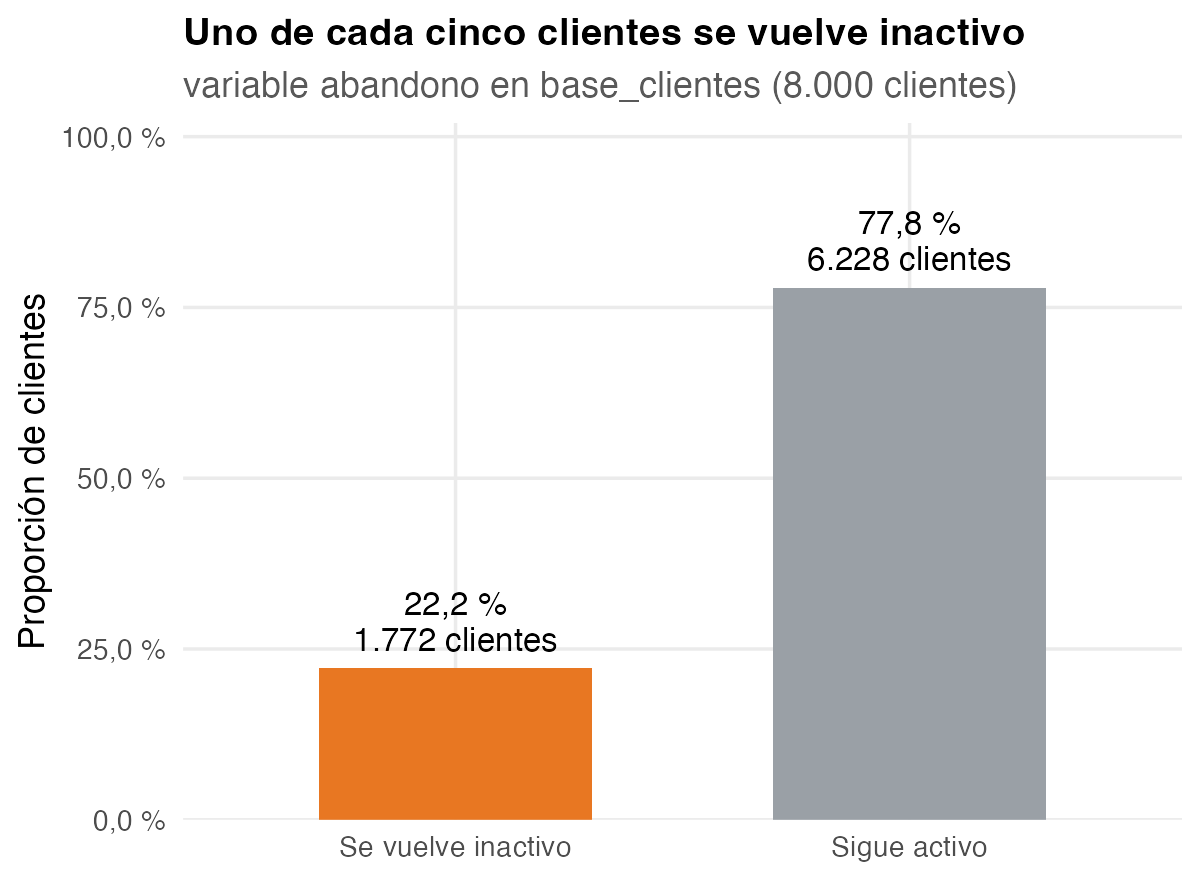
\includegraphics[width=\textwidth]{pic/fig_target.png}
\column{0.48\textwidth}
\begin{itemize} \itemsep5pt
  \item \textbf{1.772 de 8.000 = 22,15\,\%.} Esa es la \textbf{tasa base}: el punto de comparación de todo lo que sigue.
  \item Desbalance moderado: la métrica del modelo \emph{no} podrá ser la exactitud a secas (semana 10).
  \item \textbf{¿Qué es ``activo''?} 886 clientes llevan \textbf{más de 90 días} sin transar; el 59,7\,\% de ellos ya está marcado como abandono. ¿Son ``clientes activos hoy''?
\end{itemize}
\end{columns}
\pause
\vspace{0.1cm}
\begin{alertblock}{La decisión del paso}
La definición de ``activo'' se acuerda \textbf{con Growth antes de modelar} (¿recencia $\leq$ 90 días?). El abismo semántico del podcast también existe \emph{dentro} de la empresa.
\end{alertblock}
\end{frame}

%%=================================================
\begin{frame}{Paso 4 · ¿Cómo se distribuyen las candidatas?}
\small
\begin{columns}[T]
\column{0.5\textwidth}
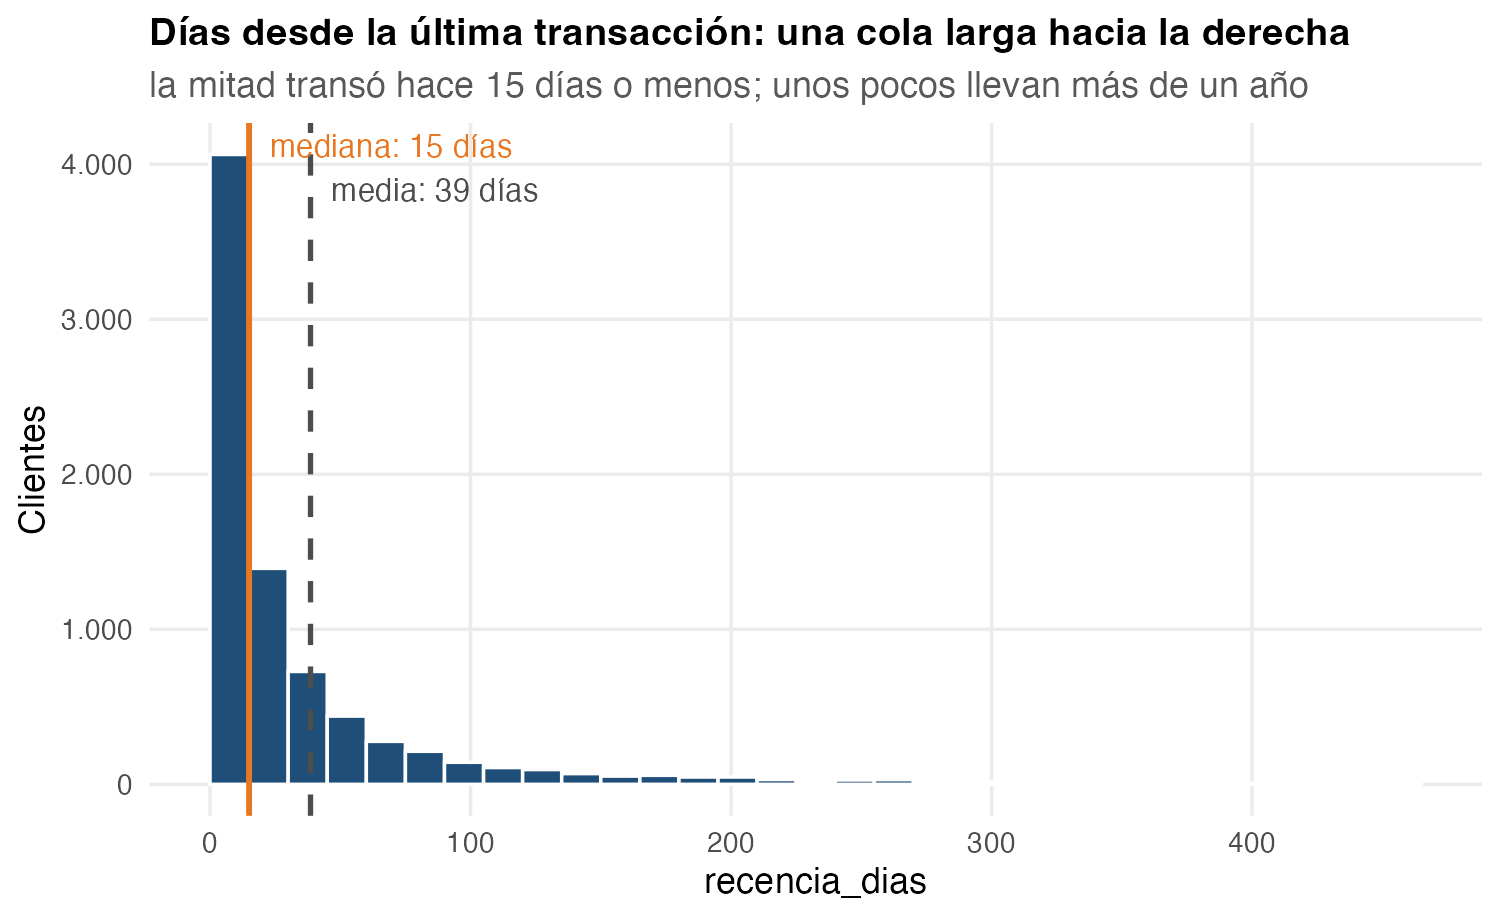
\includegraphics[width=0.96\textwidth]{pic/fig_recencia_hist.png}
\column{0.5\textwidth}
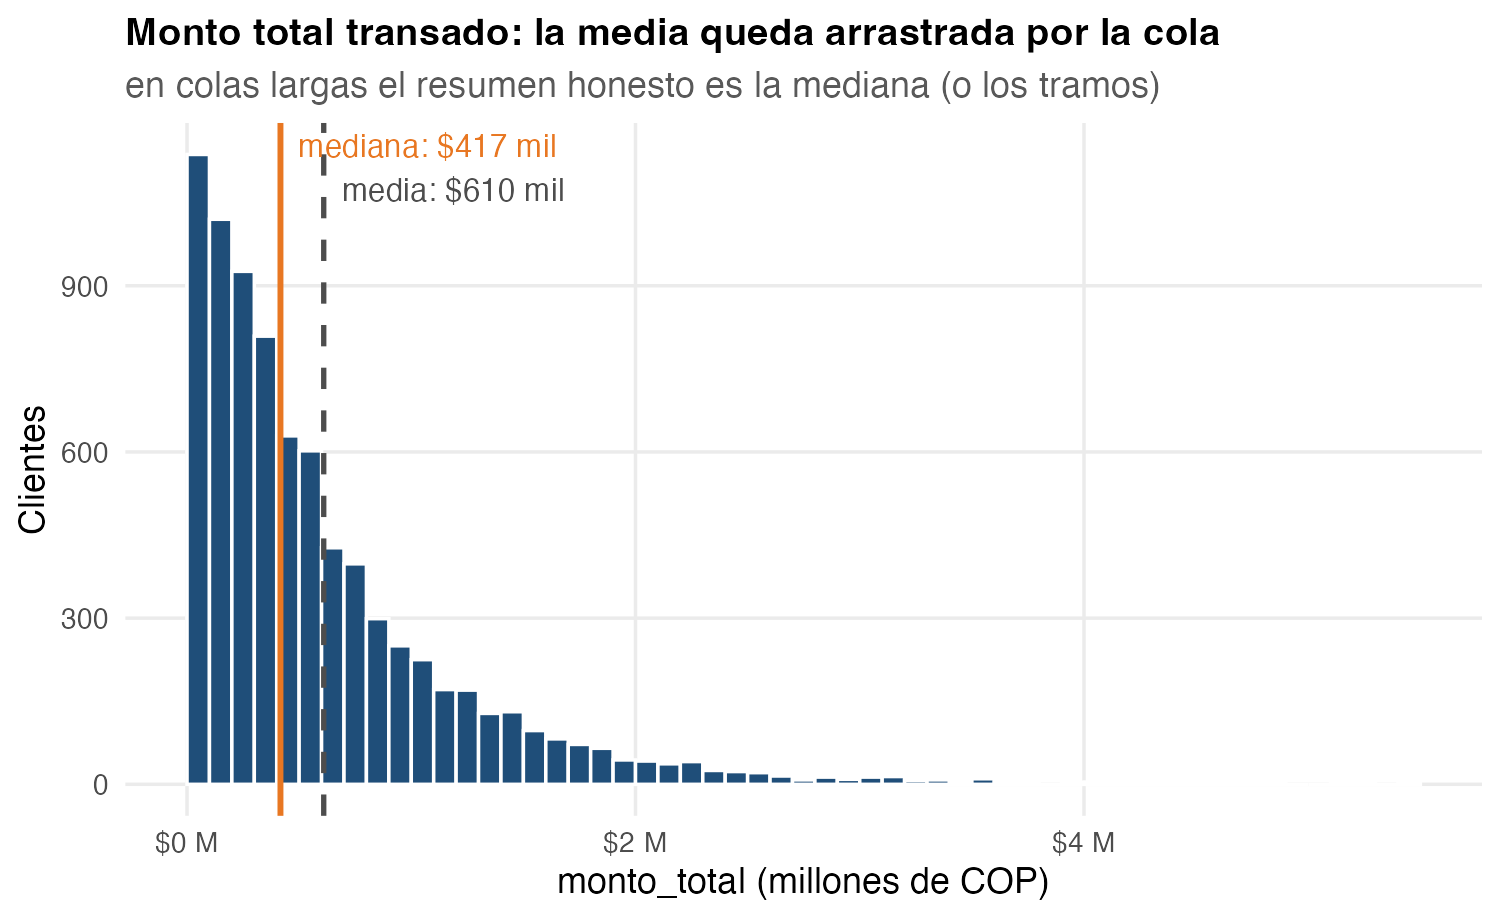
\includegraphics[width=0.96\textwidth]{pic/fig_monto_hist.png}
\end{columns}

\vspace{0.1cm}
\begin{itemize} \itemsep2pt
  \item Las dos tienen \textbf{cola larga a la derecha} y la media queda arrastrada: recencia, mediana \textbf{15} días vs.\ media \textbf{39}; monto total, mediana \textbf{\$417 mil} vs.\ media \textbf{\$610 mil}. ``El cliente promedio transó hace 39 días'' describe a muy pocos.
\end{itemize}
\pause
\begin{block}{La decisión del paso}
Describir con \textbf{medianas y tramos}, no con promedios. Las comparaciones del paso 5 se hacen por tramos.
\end{block}
\end{frame}

%%=================================================
\begin{frame}{Paso 5 · ¿Quiénes abandonan más?}
\small
\begin{columns}[T]
\column{0.5\textwidth}
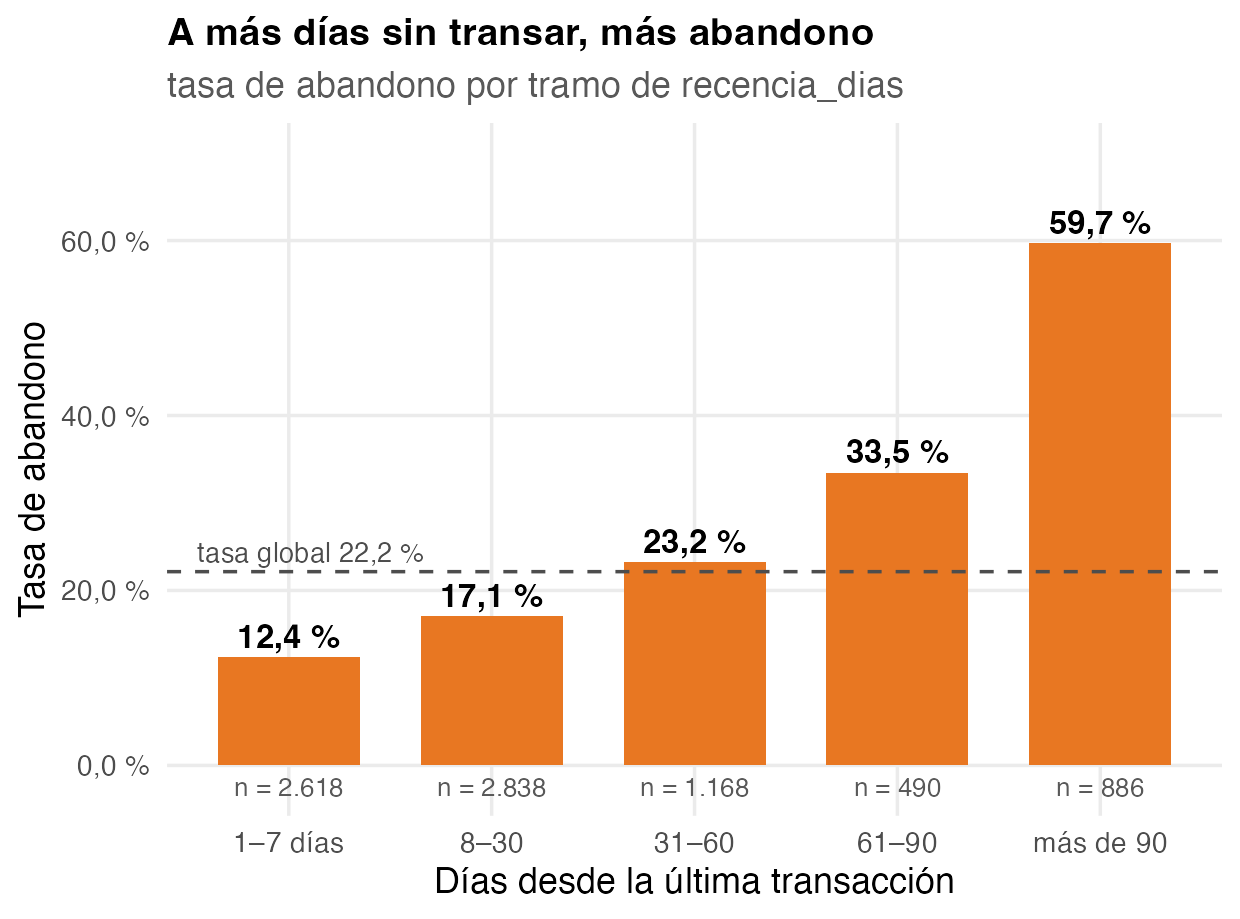
\includegraphics[width=0.9\textwidth]{pic/fig_abandono_recencia.png}
\column{0.5\textwidth}
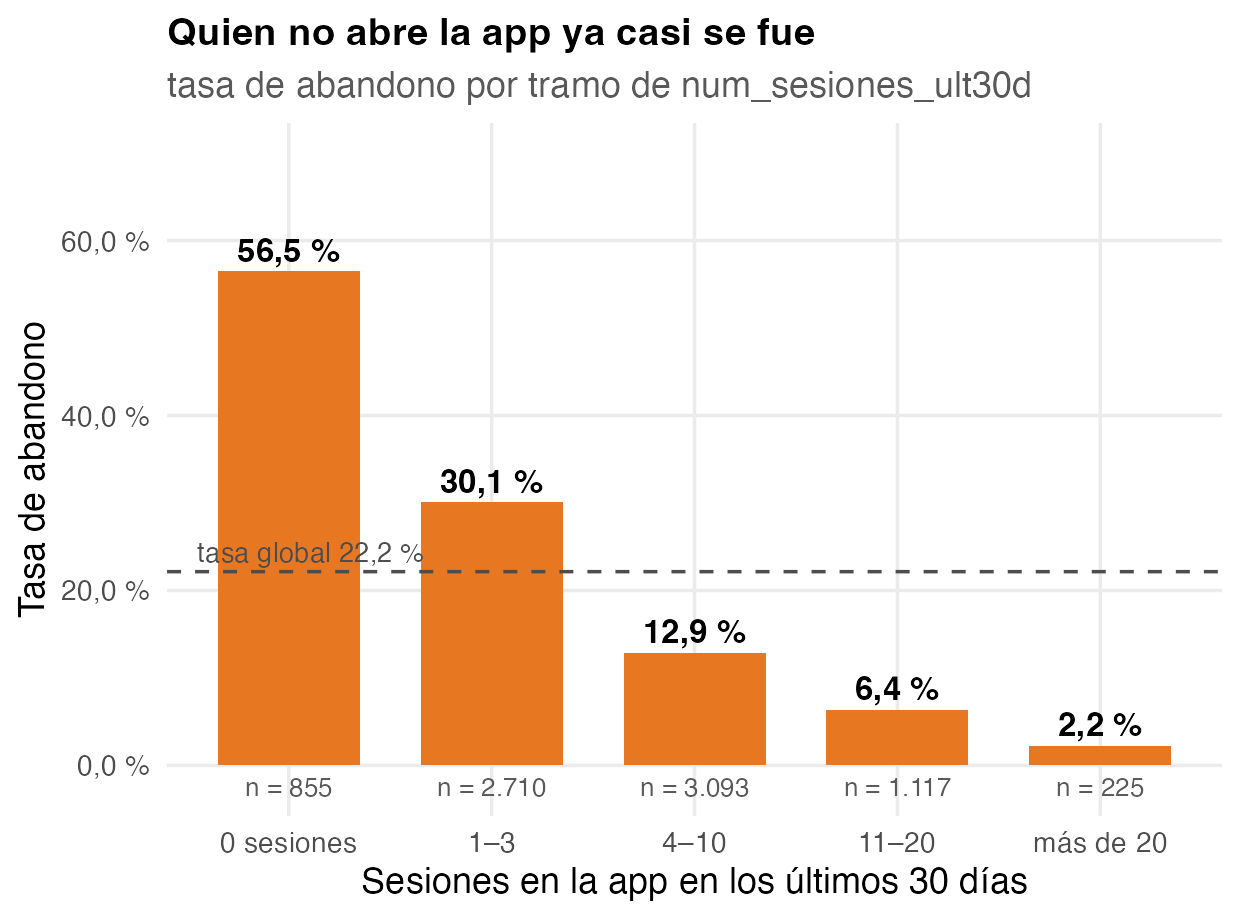
\includegraphics[width=0.9\textwidth]{pic/fig_abandono_sesiones.png}
\end{columns}

\vspace{0.05cm}
\begin{itemize} \itemsep2pt
  \item Recencia: del \textbf{12,4\,\%} (transó esta semana) al \textbf{59,7\,\%} (más de 90 días). Sesiones: del \textbf{56,5\,\%} (cero) al \textbf{2,2\,\%} (más de 20). La línea punteada es la tasa global: importa \textbf{cuánto se aleja} cada tramo.
\end{itemize}
\pause
\begin{alertblock}{Hallazgo 1}
El \textbf{comportamiento reciente} es la señal. Y el ``faltante'' del paso 2 --- cero sesiones --- resultó ser el grupo de mayor riesgo de toda la base.
\end{alertblock}
\end{frame}

%%=================================================
\begin{frame}{Paso 6 · ¿Y lo que ``debería'' importar?}
\small
\begin{columns}[T]
\column{0.5\textwidth}
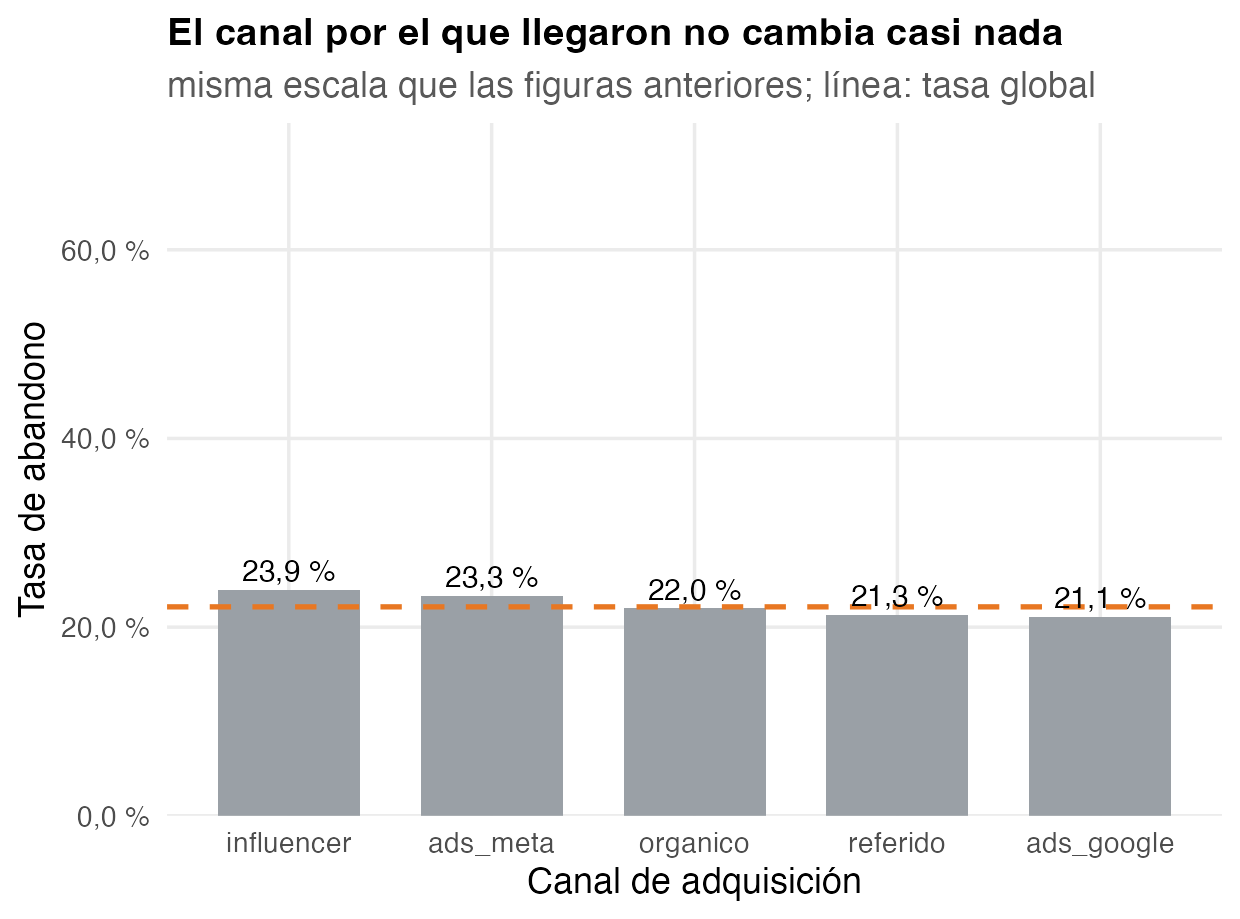
\includegraphics[width=0.82\textwidth]{pic/fig_abandono_canal.png}
\column{0.5\textwidth}
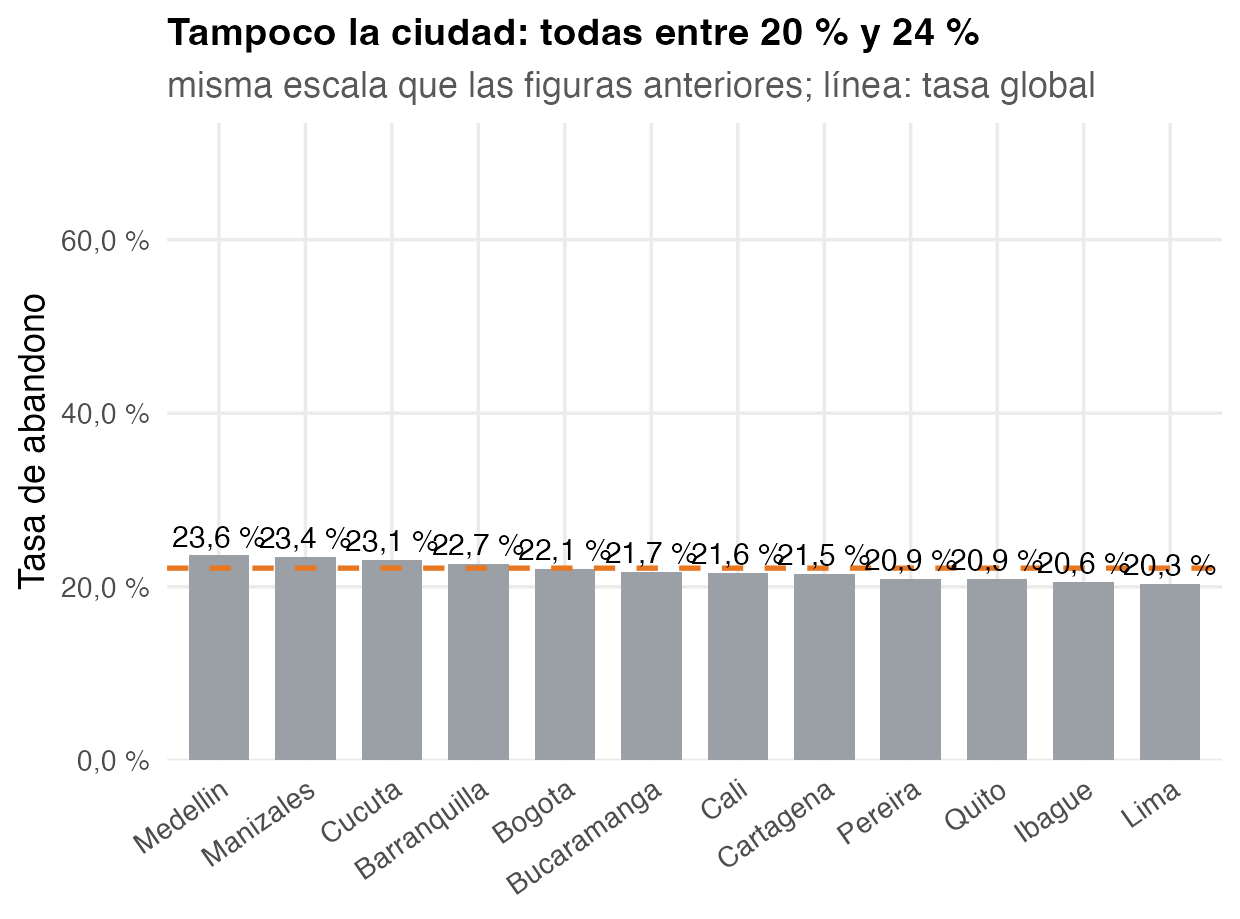
\includegraphics[width=0.82\textwidth]{pic/fig_abandono_ciudad.png}
\end{columns}

\vspace{0.05cm}
\begin{itemize} \itemsep2pt
  \item Misma escala que la lámina anterior, a propósito. Canal: \textbf{21,1 a 23,9\,\%}; ciudad: \textbf{20,3 a 23,6\,\%}; género, sistema operativo, KYC y ocupación: todo entre 20 y 25\,\%. ``Los de \emph{influencer} se van más'' es ruido alrededor de la tasa global.
\end{itemize}
\pause
\begin{alertblock}{Hallazgo 2 --- un gráfico plano también es un hallazgo}
La demografía y el canal \textbf{no discriminan}: la campaña se segmenta por comportamiento, no por ciudad ni por canal.
\end{alertblock}
\end{frame}

%%=================================================
\begin{frame}{Paso 7 · ¿Las dos señales miden lo mismo?}
\small
\begin{center}
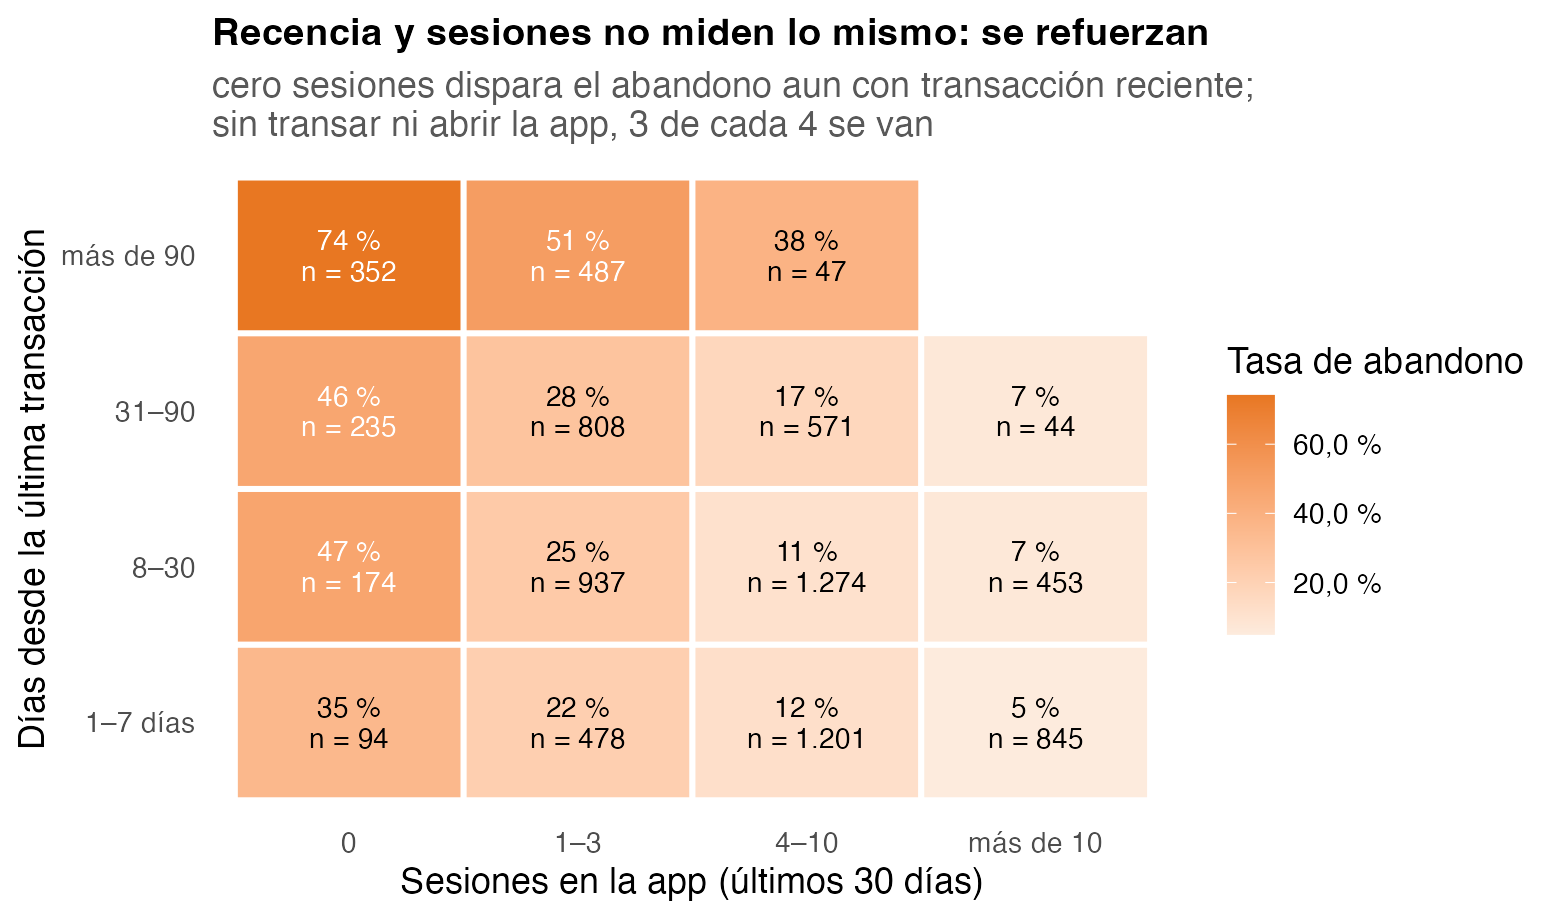
\includegraphics[width=0.64\textwidth]{pic/fig_cruce.png}
\end{center}
\vspace{-0.15cm}
\begin{itemize} \itemsep2pt
  \item Correlación recencia--sesiones: \textbf{$-$0,35}. Se parecen, pero no son lo mismo: con transacción de esta semana y \textbf{cero sesiones}, el abandono ya es del 35\,\%; sin transar en 90 días y sin sesiones, \textbf{74\,\%}; con más de 10 sesiones nunca pasa del 7\,\%.
\end{itemize}
\begin{block}{La decisión del paso}
Las dos señales entran a la base analítica; la campaña ya sabe a quién ir primero (arriba a la izquierda).
\end{block}
\end{frame}

%%=================================================
\begin{frame}{Paso 8 · ¿Qué aporta un anexo? Agregar y luego unir}
\small
\begin{columns}[T]
\column{0.52\textwidth}
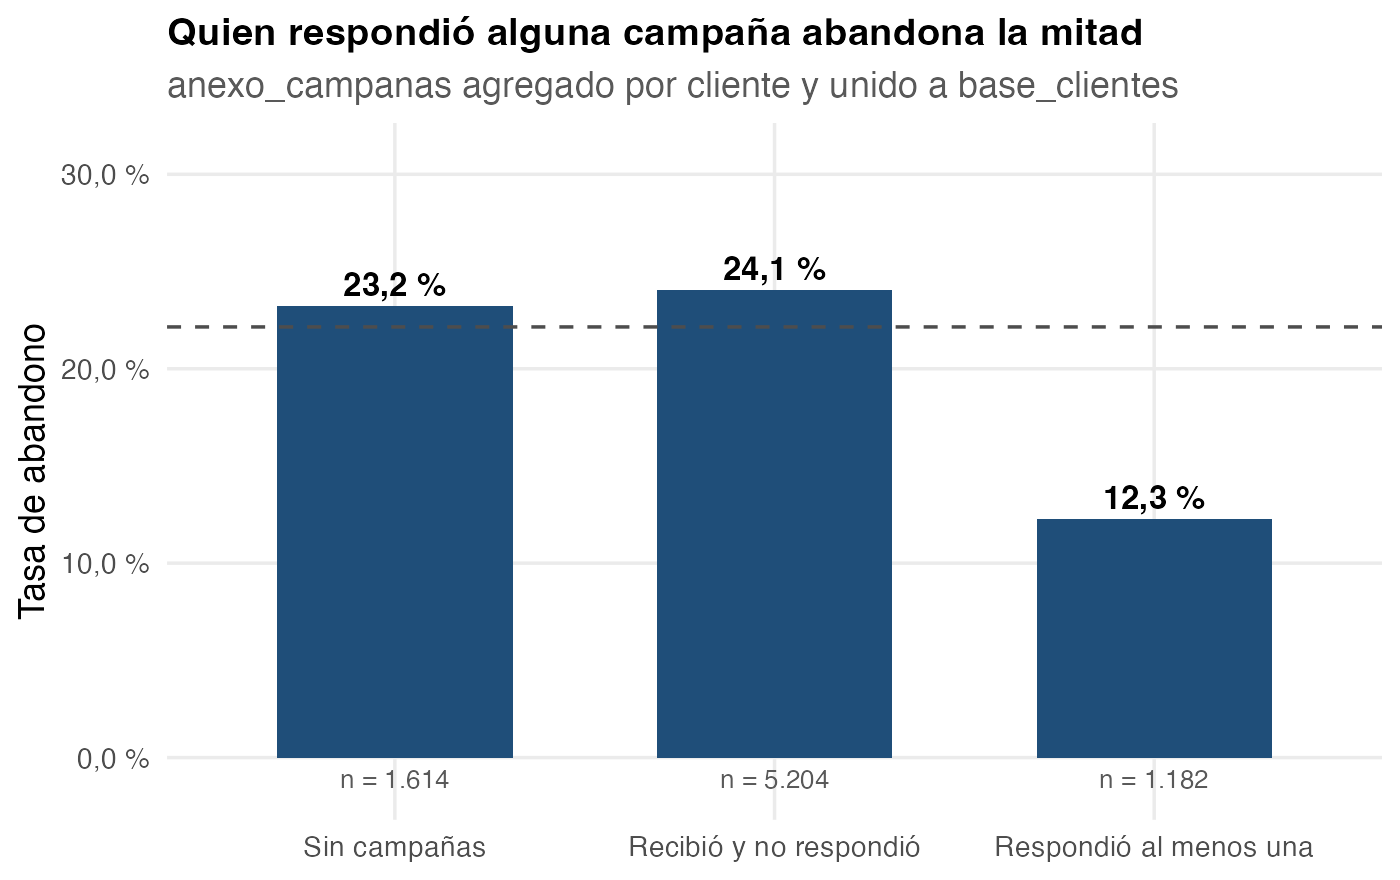
\includegraphics[width=\textwidth]{pic/fig_campanas.png}
\column{0.46\textwidth}
\footnotesize
\textbf{El grano, en vivo:}
\begin{itemize} \itemsep3pt
  \item \texttt{anexo\_campanas}: 13.467 envíos a 6.386 clientes.
  \item Se \textbf{agrega} por cliente (\texttt{n\_campanas}, \texttt{n\_convertidas}) y \emph{después} se une a la base: siguen siendo \textbf{8.000 filas}.
  \item Unido \textbf{sin agregar}: \textbf{15.081 filas}. Clientes duplicados, totales inflados, y R no dice nada.
  \item 1.614 clientes nunca recibieron campaña: tras el \texttt{join} quedan en \texttt{NA} $\to$ se vuelven 0 y se documenta.
\end{itemize}
\end{columns}
\pause
\vspace{0.05cm}
\begin{alertblock}{Hallazgo 3 --- con letra pequeña}
Quien respondió alguna campaña abandona el \textbf{12,3\,\%} frente al \textbf{24,1\,\%}. Pero es \textbf{correlación}: ¿la campaña retiene, o los clientes fieles responden más? Es una hipótesis para el modelo, no una conclusión para Growth.
\end{alertblock}
\end{frame}

%%=================================================
\begin{frame}{Paso 9 · ¿Qué raro quedó --- y qué \emph{no} puedo usar?}
\small
\begin{columns}[T]
\column{0.5\textwidth}
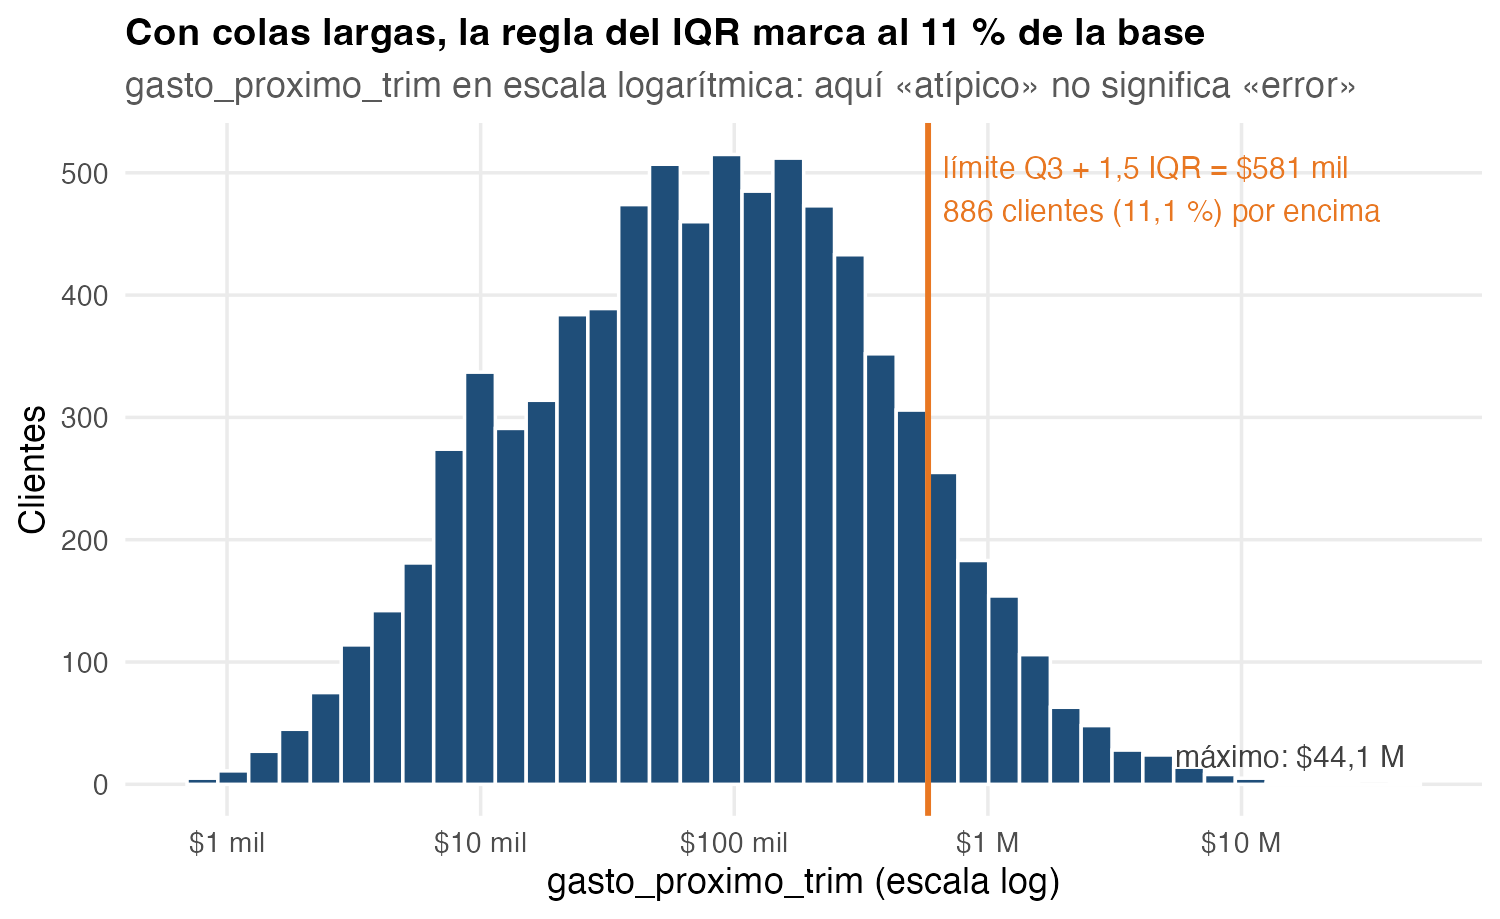
\includegraphics[width=\textwidth]{pic/fig_gasto_cola.png}
\column{0.48\textwidth}
\footnotesize
\begin{itemize} \itemsep2pt
  \item La regla del IQR marca \textbf{886 clientes (11\,\%)}. En una cola larga, ``atípico'' no significa ``error'': significa que la regla no aplica.
  \item El máximo, \textbf{\$44,1 millones}: se mira la fila completa. Cliente de \textbf{1 mes}, \textbf{72 transacciones}, transó \textbf{ayer}, 15 sesiones. No es un dedo de más: es un cliente que despegó. \textbf{Se conserva y se reporta.}
\end{itemize}
\end{columns}
\pause
\begin{alertblock}{La fuga de información (la regla de oro del caso)}
\texttt{gasto\_proximo\_trim} ``predice'' el abandono de maravilla: mediana de \$105 mil en quienes se quedan y \$23 mil en quienes se van. Claro: \textbf{es el futuro}, se conoce después del corte igual que \texttt{abandono}. Nunca entra como predictor. Cuando una variable predice demasiado bien, sospechen de esto.
\end{alertblock}
\end{frame}

%%=================================================
%% SECCIÓN 3: LO QUE SALE
%%=================================================
\section{Lo que sale del EDA}

\begin{frame}[noframenumbering]{Roadmap}
\tableofcontents[currentsection]
\end{frame}

%%=================================================
\begin{frame}{El EDA de hoy, en una lámina}
\footnotesize
\begin{columns}[T]
\column{0.5\textwidth}
\textbf{Hallazgos (con número)}
\begin{enumerate} \itemsep1pt
  \item 22\,\% de los clientes se vuelve inactivo; el comportamiento reciente separa tasas del 5\,\% al 74\,\%.
  \item Demografía, ciudad y canal no discriminan: todo entre 20 y 25\,\%.
  \item Quien respondió alguna campaña abandona la mitad (12 vs.\ 24\,\%).
\end{enumerate}
\vspace{0.1cm}
\textbf{Hipótesis para el modelo}
\begin{itemize} \itemsep1pt
  \item Priorizar la reactivación en \textbf{cero sesiones y más de 30 días sin transar}: 587 clientes con tasas del 46 al 74\,\%.
  \item La respuesta a campañas puede ser causa o síntoma: señal, no palanca.
\end{itemize}
\column{0.48\textwidth}
\textbf{Decisiones (el acta)}
\begin{itemize} \itemsep1pt
  \item Faltantes = ``no aplica'' $\to$ indicadores; nada se imputa.
  \item Definir ``activo'' con Growth (¿recencia $\leq$ 90 días?) antes de modelar.
  \item Fuera de la base analítica: \texttt{gasto\_proximo\_trim} (es del futuro).
  \item Anexos: agregar por cliente antes de unir; verificar que sigan 8.000 filas.
  \item El máximo de \$44,1 M se conserva y se reporta.
\end{itemize}
\vspace{0.1cm}
\begin{block}{\footnotesize La base analítica}
\footnotesize 8.000 filas $\times$ lo que la pregunta necesita: target, recencia, sesiones, RFM, indicadores derivados y campañas agregadas.
\end{block}
\end{columns}
\end{frame}

%%=================================================
\begin{frame}{Qué produce un EDA --- y qué no}
\small
Lo de hoy, generalizado. De cualquier EDA hecho \textbf{con una pregunta} se sale con cuatro cosas:

\vspace{0.1cm}
\begin{enumerate} \setlength{\itemsep}{0.18cm}
  \item \textbf{Hallazgos con número}, en lenguaje de negocio: ``los clientes sin sesiones en 30 días abandonan el 56\,\%'' --- no ``la variable sesiones es significativa''.
  \item \textbf{Hipótesis} para el modelo: qué señales prometen, cuáles salieron planas y qué habría que confirmar.
  \item \textbf{Decisiones documentadas} (el acta): qué se hizo con los faltantes y los extremos, qué columnas se derivaron y cuáles se excluyeron --- con el porqué.
  \item \textbf{Una base analítica} lista: una fila por unidad de análisis, con lo que la pregunta necesita y sin lo que se conoce después del corte.
\end{enumerate}
\pause
\vspace{0.1cm}
\begin{alertblock}{Y con lo que no se sale}
Ni con la respuesta a la pregunta de negocio, ni con un modelo, ni con un catálogo de gráficos: hoy fueron nueve pasos y diez figuras para 29 columnas. Si una figura no acerca a la decisión, no va.
\end{alertblock}
\end{frame}

\end{document}
